\documentclass[12pt]{article}

\usepackage[margin=1in]{geometry}
\usepackage{enumitem}
\usepackage{graphicx}

\graphicspath{{./img/}}

\begin{document}
	\begin{center}
		\begin{large}
			Computer Networks Homework 1
		\end{large}
	\end{center}
	
	\hfill Charlie Coleman
	
	\noindent \textbf{Question 1}
	
	\begin{enumerate}[nolistsep]
		\item \begin{enumerate} [nolistsep]
			\item A network protocol defines the format and order of messages exchanged between two or more communicating devices on a network, as well as the actions taken on the transmission and/or receipt of a message.
			\item A network service is an application running at or above the application layer. Can serve many different functions, like data storage, presentation, etc.
			\item Service interface - theoretical, a definition of the service independent of implementation
			
			Implementation of a service - practical, follows the service interface definition and implements the service
		\end{enumerate}
		\item \begin{enumerate}
			\item A network architecture - framework for the specs of a network's physical components \& functional org/config, operation principles \& procedures, \& communication protocols
			\item ISO/OSI - Application, Presentation, Session, Transport, Network, Link, Physical layers
			
			TCP/IP - Application, Transport, Network, Data Link, Physical layers
		\end{enumerate}
		\item \begin{enumerate}
			\item[1k)] Overhead: $100*1,000,000/1,000 = 100,000$ bytes

			Bytes lost: 1 packet AKA 1,000 bytes
			
			Total: 101,000 bytes
			\item[5k)] Overhead: $100*1,000,000/5,000 = 20,000$ bytes
			
			Bytes lost: 1 packet AKA 5,000 bytes
			
			Total: 25,000 bytes
			\item[\textbf{10k)}] Overhead: $100*1,000,000/10,000 = 10,000$ bytes
			
			Bytes lost: 1 packet AKA 10,000 bytes
			
			\textbf{Total: 20,000 bytes (OPTIMAL)}
			\item[20k)] Overhead: $100*1,000,000/20,000 = 5,000$ bytes
			
			Bytes lost: 1 packet AKA 20,000 bytes
			
			Total: 25,000 bytes
		\end{enumerate}
	\end{enumerate}
	
	\noindent \textbf{Question 2}
	
	\begin{enumerate}[nolistsep]
		\item Recording on eno1, my PC is connected via ethernet to the SLU network
		\item Protocols
		
		\begin{itemize}[nolistsep, noitemsep]
			\item TCP - transport layer
			\item TLSv1.2/3 - presentation layer
		\end{itemize}
		\item 
		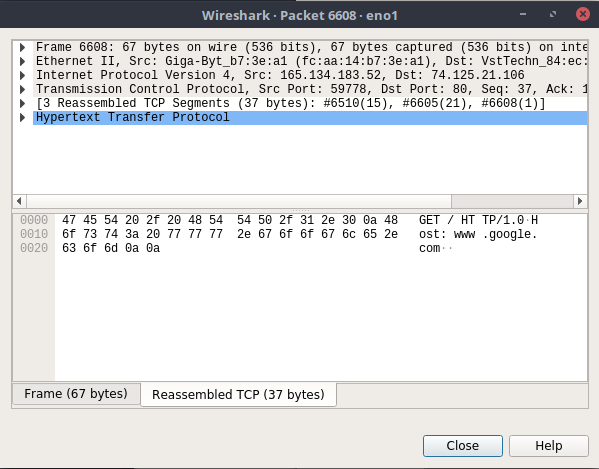
\includegraphics[height=4in]{2c}
	\end{enumerate}
	
	\noindent \textbf{Question 3}
	
	\begin{enumerate}[nolistsep]
		\item Traceroute uses the IP TTL field to cause an ICMP TIME\_EXCEEDED response from each gateway. Firewalls filter the "unlikely" UDP ports, or the ICMP echoes.\\
		\item \begin{tabular}{|l|l|l|}
			\hline
			& First Round & Second Round \\
			\hline
			Trial 1 & 30.856ms & 79.627ms \\
			Trial 2 & 31.305ms & 79.249ms \\
			Trial 3 & 30.942ms & 78.053ms \\
			Trial 4 & 31.624ms & 78.726ms \\
			Trial 5 & 30.936ms & 77.228ms \\
			\hline
			Average & 31.1326ms & 78.5766ms \\
			Std Deviation & 0.32507ms & 0.9579ms \\
			\hline			
		\end{tabular}
		~\\
		\item 165.134.183.254, 165.134.198.4, 165.134.248.137, 10.248.101.30, 10.248.100.20, 165.134.223.27, 10.248.5.2, 34.230.135.168\\
		
		165.134.183.254 - St. Louis University
		
		165.134.198.4 - St. Louis University

		165.134.248.137 - St. Louis University
		
		10.248.101.30 - Private IP Address LAN
		
		10.248.100.20 - Private IP Address LAN
		
		165.134.223.27 - SLU
		
		10.248.5.2- No ISP associated 
		
		34.230.135.168 - Amazon.com, Inc.
	\end{enumerate}
\end{document}